\documentclass[prd,twocolumn,superscriptaddress,nofootinbib,floatfix]{revtex4-2}
\usepackage{amsmath,amssymb,graphicx,booktabs,xcolor,hyperref}
\hypersetup{colorlinks=true,linkcolor=blue!50!black,citecolor=blue!50!black,urlcolor=blue!50!black}
% Numbers quoted in the text. DRAFT: filled by hand from results/ for now; to be generated
% by a script from the results files once all phases have run.
\newcommand{\NphaseZeroWorst}{1.1\times10^{-3}}
\newcommand{\NlosRefWorst}{7.7\times10^{-3}}
\newcommand{\pending}[1]{\textcolor{red!70!black}{[\textbf{Pending:} #1]}}


\newcommand{\kd}{\dot\kappa}
\newcommand{\Hc}{\mathcal{H}}
\newcommand{\taurec}{\tau_{\rm rec}}

\begin{document}

\title{Data-free physics-informed neural networks for the linear Einstein--Boltzmann equations of the cosmic microwave background}

\author{[Author names]}
\affiliation{[Affiliations]}

\begin{abstract}
\textbf{[Draft abstract; final numbers pending.]} We present a physics-informed neural network (PINN) that solves the linearised Einstein--Boltzmann equations of the photon--baryon--dark-matter--neutrino system in conformal Newtonian gauge without any training data: the networks are trained only on the residuals of the equations. We identify the ingredients without which training fails or converges to wrong solutions, each isolated in controlled experiments: initial conditions that satisfy the Einstein $00$ constraint, the $00$ residual as a loss term (which removes a constraint-violating solution that otherwise grows like conformal time), time-dependent physical scaling of the outputs, preconditioning of the stiff Thomson-scattering equations with a slow-manifold hand-over at the tight-coupling switch, and time-marching over a chain of networks (a single network collapses to a trivial solution once modes oscillate). With these, single modes reach $10^{-4}$--$10^{-3}$ accuracy against a stiff ODE solver through several acoustic oscillations, and a bundle over wavenumber reaches an RMS error of $\sim10^{-3}$ in the tight-coupling era. \pending{accuracy through recombination, $C_\ell^{TT}$ vs \textsc{class}, parameter bundle, and the beyond-$\Lambda$CDM inverse problem.}

\end{abstract}

\maketitle

%=====================================================================================
\section{Introduction}
%=====================================================================================

Predictions for cosmic microwave background (CMB) anisotropies rest on the linearised Einstein--Boltzmann equations, solved for every Fourier mode by codes such as \textsc{camb}~\cite{CAMB} and \textsc{class}~\cite{CLASS1,CLASS2}. Two developments have changed how these predictions are used. Neural emulators~\cite{CosmicNet1,CosmicNet2,CosmoPower,CosmoPowerJAX} replace a Boltzmann code by a network trained on its outputs, and differentiable Boltzmann codes~\cite{DISCOEB,SymBoltz,ABCMB} provide exact gradients of observables with respect to parameters. Emulators are fast but need a solver to produce training data, which ties them to models that some code already implements. Differentiable solvers are exact but solve one cosmology at a time.

Physics-informed neural networks (PINNs)~\cite{Lagaris1998,Raissi2019} sit between the two. A PINN is trained on the residual of the governing equations rather than on solutions, so it needs no training data, and a single network can represent a whole family of solutions when the parameters are network inputs (a ``bundle''~\cite{Flamant2020}). In cosmology PINN bundles have so far been applied to the background expansion~\cite{Chantada2023,Chantada2024} and to the sub-horizon growth equation for matter, a single second-order ODE~\cite{GomezBachar2025}. The latter work describes itself as a first step towards the coupled Boltzmann system. Related neural approaches solve the homogeneous Boltzmann equations of particle decoupling~\cite{NBE}. To our knowledge no PINN has been applied to the coupled photon--baryon--dark-matter--neutrino perturbation system that determines the CMB.

This system is a hard test for PINNs. It is stiff (Thomson scattering is $10^{3}$--$10^{9}$ times faster than the expansion before recombination), multi-scale (the integration covers seven decades in conformal time and the variables span many orders of magnitude), oscillatory (acoustic waves and free streaming), and it carries a constraint (the Einstein $00$ equation) that the evolution equations propagate but do not enforce. This paper asks whether a data-free PINN can nevertheless reach the accuracy needed for CMB predictions, and documents what it takes.

Our contributions are:
\begin{enumerate}
\item A data-free PINN for the full linear system in conformal Newtonian gauge: tight-coupled photon--baryon fluid, the photon temperature and polarisation hierarchies with Thomson scattering, massless neutrinos, cold dark matter, and the metric. The network is trained as a bundle over wavenumber, and over $(\omega_b,\omega_c)$ in the tight-coupling era.
\item A set of ingredients without which the training fails, each isolated in controlled experiments (Sec.~\ref{sec:pilots}): constraint-consistent initial conditions, the Einstein $00$ residual as a loss term, time-dependent physical scaling of the outputs, Thomson-row preconditioning with a slow-manifold hand-over at the tight-coupling switch, and time-marching over a chain of networks.
\item Line-of-sight CMB temperature spectra $C_\ell^{TT}$ computed from PINN source functions, validated against \textsc{class}.
\item A demonstration outside $\Lambda$CDM: a bundle over a late-time modification of the effective Newton constant for perturbations, used as a data-free, differentiable emulator in an inverse problem.
\end{enumerate}
We report all accuracy against an independent stiff ODE solver that integrates exactly the same equations, so that PINN error and modelling error are separated, and against \textsc{class}. We also report where the method falls short of its targets and what it costs.

%=====================================================================================
\section{Equations and reference solutions}\label{sec:equations}
%=====================================================================================

\subsection{Perturbation equations}
We work in conformal Newtonian gauge, $ds^2=a^2[-(1+2\psi)d\tau^2+(1-2\phi)d\mathbf{x}^2]$, with the variables and conventions of Ma \& Bertschinger~\cite{MaBertschinger1995} (MB95): density contrasts $\delta_i$, velocity divergences $\theta_i$, anisotropic stresses $\sigma_i$, and Legendre moments $F_{\gamma\ell}$, $G_{\gamma\ell}$, $F_{\nu\ell}$ of the photon intensity, photon polarisation and massless-neutrino distributions, truncated at $\ell_{\max}$ with the MB95 scheme. The metric is evolved with the $0i$ Einstein equation,
\begin{equation}
\dot\phi = -\Hc\psi + \frac{4\pi G a^2}{k^2}\sum_i(\bar\rho_i+\bar P_i)\theta_i ,\label{eq:phidot}
\end{equation}
and $\psi$ follows algebraically from the traceless $ij$ equation, $k^2(\phi-\psi)=12\pi G a^2\sum_i(\bar\rho_i+\bar P_i)\sigma_i$. The $00$ equation,
\begin{equation}
C_{00}\equiv k^2\phi+3\Hc(\dot\phi+\Hc\psi)+4\pi G a^2\delta\rho = 0 ,\label{eq:c00}
\end{equation}
is not used for evolution; we report it normalised by the sum of the magnitudes of its three terms. CDM, baryons, photons and neutrinos obey the MB95 equations (eqs.~30, 50, 64--65 of the arXiv version, with the baryon equation of their \S5.6). Before recombination we use the zeroth-order tight-coupling approximation (TCA): $\theta_b=\theta_\gamma\equiv\theta_{\gamma b}$, $\sigma_\gamma=0$, and
\begin{equation}
\dot\theta_{\gamma b}=\frac{-\Hc R\,\theta_{\gamma b}+\tfrac14 k^2\delta_\gamma+R c_s^2k^2\delta_b}{1+R}+k^2\psi ,
\end{equation}
with $R=3\bar\rho_b/4\bar\rho_\gamma$. After the TCA we evolve the full photon hierarchy with polarisation and Thomson coupling. Deep in the matter era we optionally use the radiation-streaming approximation (RSA) of \textsc{class}~\cite{CLASS2}, $\delta_{\gamma,\nu}=-4\phi$, $\theta_{\gamma,\nu}=6\dot\phi$, $\sigma=0$, switched on per mode at $\tau_R(k)=\max(45/k,\tau_{\rm fs})$ exactly as in \textsc{class}.

The background ($a$, $\Hc$, $\bar\rho_i$), the Thomson opacity $\kd=an_e\sigma_T$, the baryon sound speed, the sound horizon $r_s$ and the Silk scale $k_D$ are taken from \textsc{class} and tabulated as cubic splines that JAX~\cite{JAX} can differentiate. For the parameter bundle of Sec.~\ref{sec:phase2} we use an analytic radiation-plus-matter background that is differentiable in $(\omega_b,\omega_c)$; it agrees with \textsc{class} to $10^{-9}$ in $a$, $\Hc$ and $\bar\rho_i$ before recombination. The fiducial cosmology is Planck 2018 $\Lambda$CDM~\cite{Planck2018} with massless neutrinos ($N_{\rm eff}=3.046$) and no reionisation.

A single module implements the right-hand side $f(\tau,u;k)$ of all equations. Both the PINN residual and the reference solver call it, so any disagreement between them is a training error, not a modelling difference.

\subsection{Constraint-consistent initial conditions}\label{sec:ics}
MB95 give the adiabatic growing mode in Newtonian gauge to leading order in $k\tau$ and $\tau/\tau_{\rm eq}$. These initial conditions violate Eq.~\eqref{eq:c00} at $\mathcal{O}(\tau_i/\tau_{\rm eq})$. Evolving $\phi$ with Eq.~\eqref{eq:phidot} admits one extra solution beyond those of the full Einstein equations, along which $C_{00}\propto 1/a$; relative to the physical terms it grows like $\tau$ in the radiation era. A violation of $2\times10^{-5}$ at $\tau_i=0.01$\,Mpc grew to $5\%$ by recombination and produced 2--6\% errors in every variable compared with \textsc{class}. We therefore use the \textsc{class} initial conditions: the synchronous-gauge expansion to first order in $(k\tau)^2$ and $\omega\tau$ ($\omega=a\bar\rho_m/\sqrt{\bar\rho_r}$), followed by the gauge transformation with $\alpha=(\dot h+6\dot\eta)/2k^2$ taken from the $00$ and $0i$ equations. The initial state then satisfies Eq.~\eqref{eq:c00} to $<10^{-8}$, and reduces to MB95 eq.~98 to $2\times10^{-3}$. We verified the propagation property directly: on the constraint surface $dC_{00}/d\tau$ vanishes to $10^{-9}$ relative for both state layouts.

\subsection{Reference solver and validation against \textsc{class}}
The reference solver integrates the same right-hand side with \texttt{scipy}'s Radau method ($r_{\rm tol}=10^{-10}$ unless stated), using exact Jacobians from JAX, with the same TCA/full/RSA switches as the network. Against \textsc{class} (Newtonian gauge, matched $\ell_{\max}$, late-time approximations off) it agrees to $\le\NphaseZeroWorst$ on $\phi$, $\delta_c$, $\delta_\gamma$ for $k=0.01$ and $0.05$\,Mpc$^{-1}$ up to $2\taurec$. Without the TCA, every variable agrees to $\sim2\times10^{-4}$; the remaining difference comes from our zeroth-order TCA and vanishes linearly as the TCA switch is moved earlier.

Our line-of-sight code uses the \textsc{class} Newtonian-gauge source functions and radial functions~\cite{SeljakZaldarriaga1996}. Fed \textsc{class}'s own source functions it reproduces \textsc{class} $C_\ell^{TT}$ to $\le2\times10^{-4}$ (except $1.4\times10^{-3}$ at one multipole). Fed reference-solver sources with the \textsc{class} approximation schedule it reproduces \textsc{class} to $\le\NlosRefWorst$ for $\ell\le500$. \textsc{class} must be run with a high $\ell_{\max}$ for this comparison, because it ties its $k$ range to $\ell_{\max}$.

%=====================================================================================
\section{PINN formulation}\label{sec:method}
%=====================================================================================

\subsection{Windows, hard initial conditions and output scaling}
A window network $N$ covers $\tau\in[\tau_a,\tau_b]$ with input $x=\ln(\tau/\tau_a)/\ln(\tau_b/\tau_a)\in[0,1]$, the normalised $\ln k$, and optionally normalised cosmological parameters $\mathbf{c}$. It represents the state of one equation layout (TCA, full hierarchy or RSA) as
\begin{equation}
u(x)=u_a+\left(1-e^{-x/\epsilon}\right)S(\tau,k)\odot B(x,k,\mathbf{c}) ,\label{eq:hardic}
\end{equation}
which reproduces the window's initial state $u_a$ exactly~\cite{Lagaris1998}. $S$ is the physical magnitude of each variable. It is time-dependent: outside the horizon $\theta\propto k^2\tau$ and $F_\ell\propto(k\tau)^\ell$, rolling over at $k\tau\sim1$; photon multipoles with $\ell\ge2$ are additionally suppressed by $(k+\Hc)/(k+\Hc+\kd)$ during tight coupling; matter densities grow as $(k\tau)^2$ in the matter era. Without this scaling the loss is dominated by a $1/(k\tau)^2$ amplification in Eq.~\eqref{eq:phidot}: the initial loss was $3\times10^{11}$ and training failed. With it the initial loss is $\mathcal{O}(1)$.

$B$ is either the network output or the oscillation ansatz
\begin{equation}
B=N_0+e^{-k^2/k_D^2}\left(N_1\cos kr_s+N_2\sin kr_s\right)+N_3\cos k\tau+N_4\sin k\tau ,
\end{equation}
with smooth network heads $N_i$. The acoustic phase $kr_s$ and damping envelope carry the photon--baryon oscillations, and $k\tau$ the free-streaming phase. A related basis was used as network \emph{input} features by CosmicNet~\cite{CosmicNet1}; here it enters the output structure.

\subsection{Loss}
The loss of a window is
\begin{equation}
\mathcal{L}=\Big\langle \frac{1}{n}\sum_{i}\Big[\frac{\partial_x u_i/L-\tau f_i(\tau,u)}{S_i\,d_i}\Big]^2 + w_c\,C_{00}^2\Big\rangle ,\label{eq:loss}
\end{equation}
averaged over collocation points, with $L=\ln(\tau_b/\tau_a)$. The first term is the log-time residual of each equation in units of the variable's size. The factor $d_i=1+\tau|\partial f_i/\partial u_i|_{\rm Thomson}$ preconditions the stiff Thomson rows ($\theta_\gamma$, $\theta_b$, $F_{\gamma\ell}$, $G_{\gamma\ell}$), so that quasi-static balances are learned at $\mathcal{O}(1)$ weight. The second term is the normalised $00$ residual with $w_c=1$. It is not optional: it is the only term that penalises the constraint-violating solution of Sec.~\ref{sec:ics}. In RSA windows, and for the modified-gravity model of Sec.~\ref{sec:phase5}, the $00$ equation is not an exact consequence of the evolution equations, and we set $w_c=0$.

\subsection{Time-marching and per-mode switches}
A single network over the whole time range fails on oscillating modes (Sec.~\ref{sec:pilots}). We instead train a chain of windows in sequence. Window $j$ starts from the frozen window $j-1$ evaluated at its end, mapped between layouts where they differ. At the TCA$\to$full switch we hand over the first-order tight-coupling state: the baryon--photon slip from the quasi-static baryon Euler equation, $\sigma_\gamma=\frac{16}{45}\theta_\gamma/\kd$ and the corresponding polarisation moments. Handing over zero slip starts a transient of width $1/\kd$ that the next window cannot represent; its loss was three orders of magnitude above that of every other window. The TCA$\to$full switch is at a fixed $\tau$ at which the TCA holds for all modes in the bundle. The full$\to$RSA switch depends on $k$, and we found it must: switching all modes to the RSA at a common time ruins the low-$\ell$ spectrum (Sec.~\ref{sec:phase4}). Each mode is therefore trained in the full-hierarchy windows only up to its $\tau_R(k)$, and the RSA windows are parameterised in $\ln(\tau/\tau_R(k))$, starting from the full chain evaluated at $\tau_R(k)$.

\subsection{Training}
Each window is an MLP (4 hidden layers of 64--96 $\tanh$ units) trained with Adam (learning rate $10^{-3}$, cosine decay) on resampled collocation sets, followed by L-BFGS on a fixed, denser set. Collocation is a tensor product of stratified $\ln k$ (and Latin-hypercube parameters) with stratified window times. Training is in float64 on CPU. No reference solution enters training.

%=====================================================================================
\section{Results}\label{sec:results}
%=====================================================================================

\subsection{Controlled experiments: what makes training work}\label{sec:pilots}

We first trained single modes in the tight-coupling era, comparing each variant with the reference solver integrating the identical equations. Errors are $\max_\tau|X_{\rm PINN}-X_{\rm ref}|/\max_\tau|X_{\rm ref}|$ for each variable $X$; this metric is well defined through zero crossings, unlike pointwise relative error.

\paragraph{Output scaling.} With fixed per-variable scales the initial loss was $3\times10^{11}$ and training made no progress. The $1/(k\tau)^2$ factor in Eq.~\eqref{eq:phidot} amplifies any error in $\theta$ outside the horizon. Scaling the outputs by their super-horizon growth reduced the initial loss to $\mathcal{O}(1)$.

\paragraph{The constraint term.} At $k=0.01$\,Mpc$^{-1}$, up to $\tau=200$\,Mpc, training on the evolution residuals alone reached a lower ODE loss ($3.8\times10^{-6}$) than training with the $00$ term, yet its errors were 30 times larger: $2.7\times10^{-2}$ on $\phi$ against $9.7\times10^{-4}$ (Fig.~\ref{fig:pilot1}). Its error grows steadily after $\tau\sim10$\,Mpc, the signature of the constraint-violating solution of Sec.~\ref{sec:ics}. With the constraint term and a longer L-BFGS polish (12k steps), every variable reached $\le6\times10^{-4}$ ($\phi$: $8.5\times10^{-5}$) in 9 CPU-minutes. Causal weighting~\cite{Wang2022causal} at $\epsilon=1$ had no effect: the weights stayed $\approx1$.

\begin{figure*}
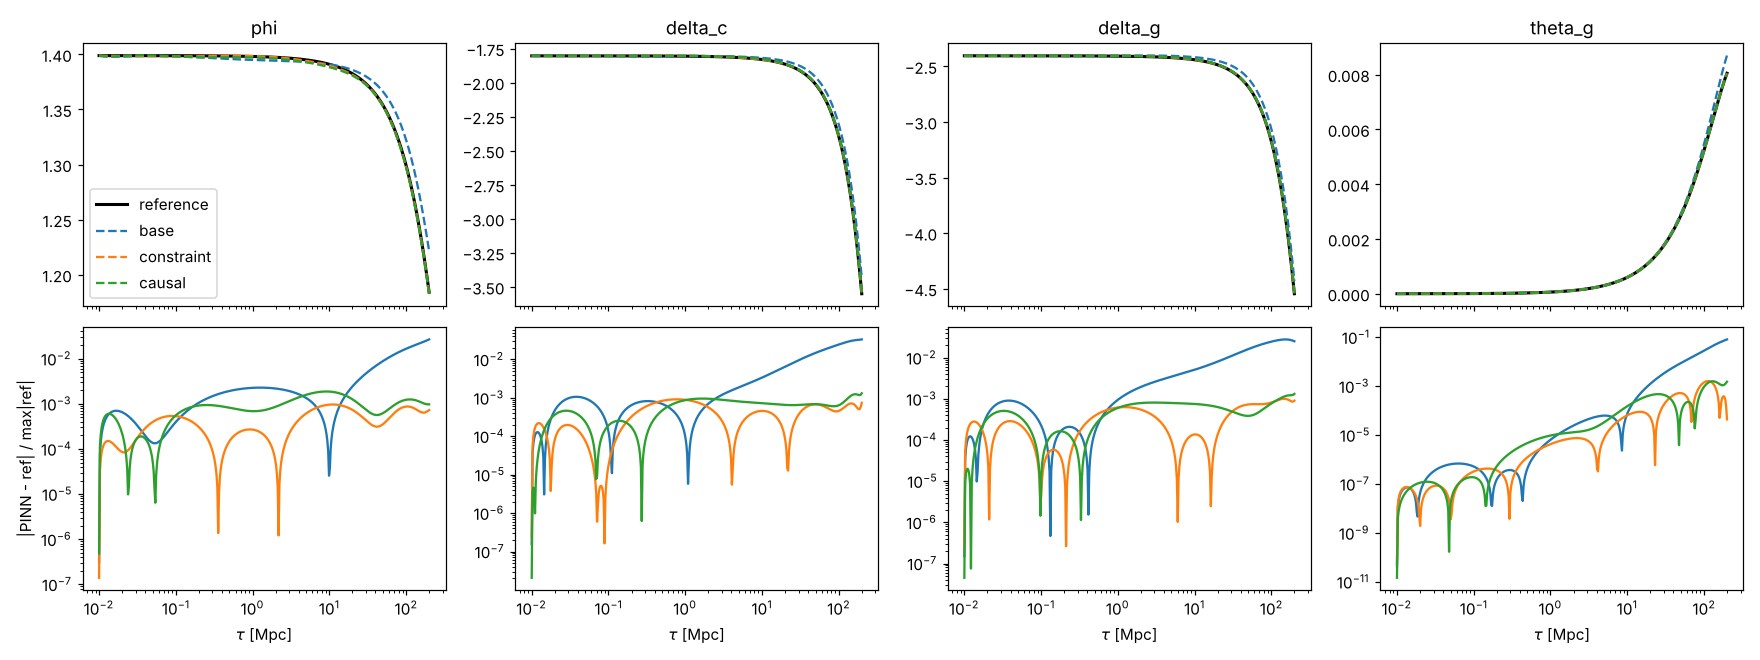
\includegraphics[width=\textwidth]{figures/pilot1.png}
\caption{Single mode $k=0.01$\,Mpc$^{-1}$, tight-coupling era. Top: PINN variants against the reference solver. Bottom: error normalised by $\max|X_{\rm ref}|$. Without the $00$ loss term (blue) the error grows steadily after $\tau\sim10$\,Mpc, despite a lower ODE residual.}
\label{fig:pilot1}
\end{figure*}

\paragraph{Oscillations and time-marching.} At $k=0.2$\,Mpc$^{-1}$, with the tight-coupling equations integrated to $\tau=200$\,Mpc (3.4 acoustic oscillations; a numerical stress test, since the TCA is not physically valid there), a single network failed with every error $\approx100\%$. It relaxed all variables towards zero from $\tau_i$ onwards (Fig.~\ref{fig:pilot2}, left), with or without the oscillation ansatz. Causal weighting at $\epsilon=10$ and $100$ did not help. This is not a problem of the equations or of capacity: the super-horizon segment alone ($\tau\le1$\,Mpc) trained to $\sim2\times10^{-3}$ at the same $k$. The single network gives up accuracy at early times to reduce the larger late-time oscillatory residual, a failure mode known for PINNs~\cite{Krishnapriyan2021}. Time-marching, with one window up to $k\tau=1$ and then one per acoustic period, chained by hard initial conditions~\cite{Wight2020,Krishnapriyan2021}, fixed it: every variable reached $\le1.0\times10^{-3}$, with no visible accumulation of error across the 8 windows (Fig.~\ref{fig:pilot2}, right). At $k=0.05$, where the TCA era holds half an oscillation, the oscillation ansatz improved a single network by $\approx2\times$.

\begin{figure*}
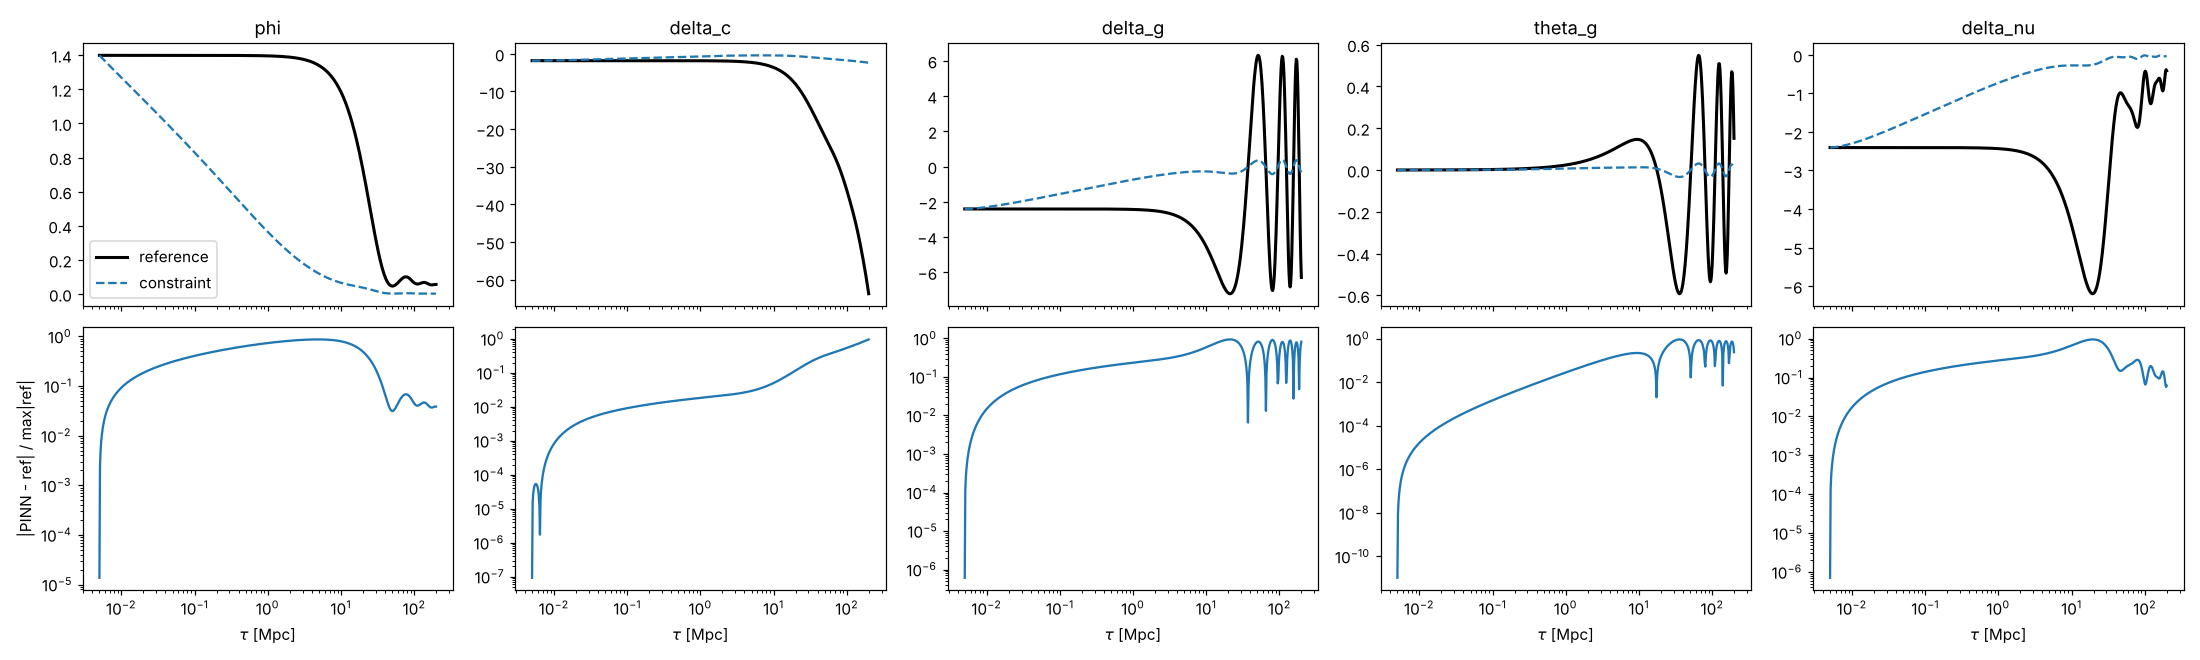
\includegraphics[width=0.49\textwidth]{figures/pilot2_single.png}\hfill
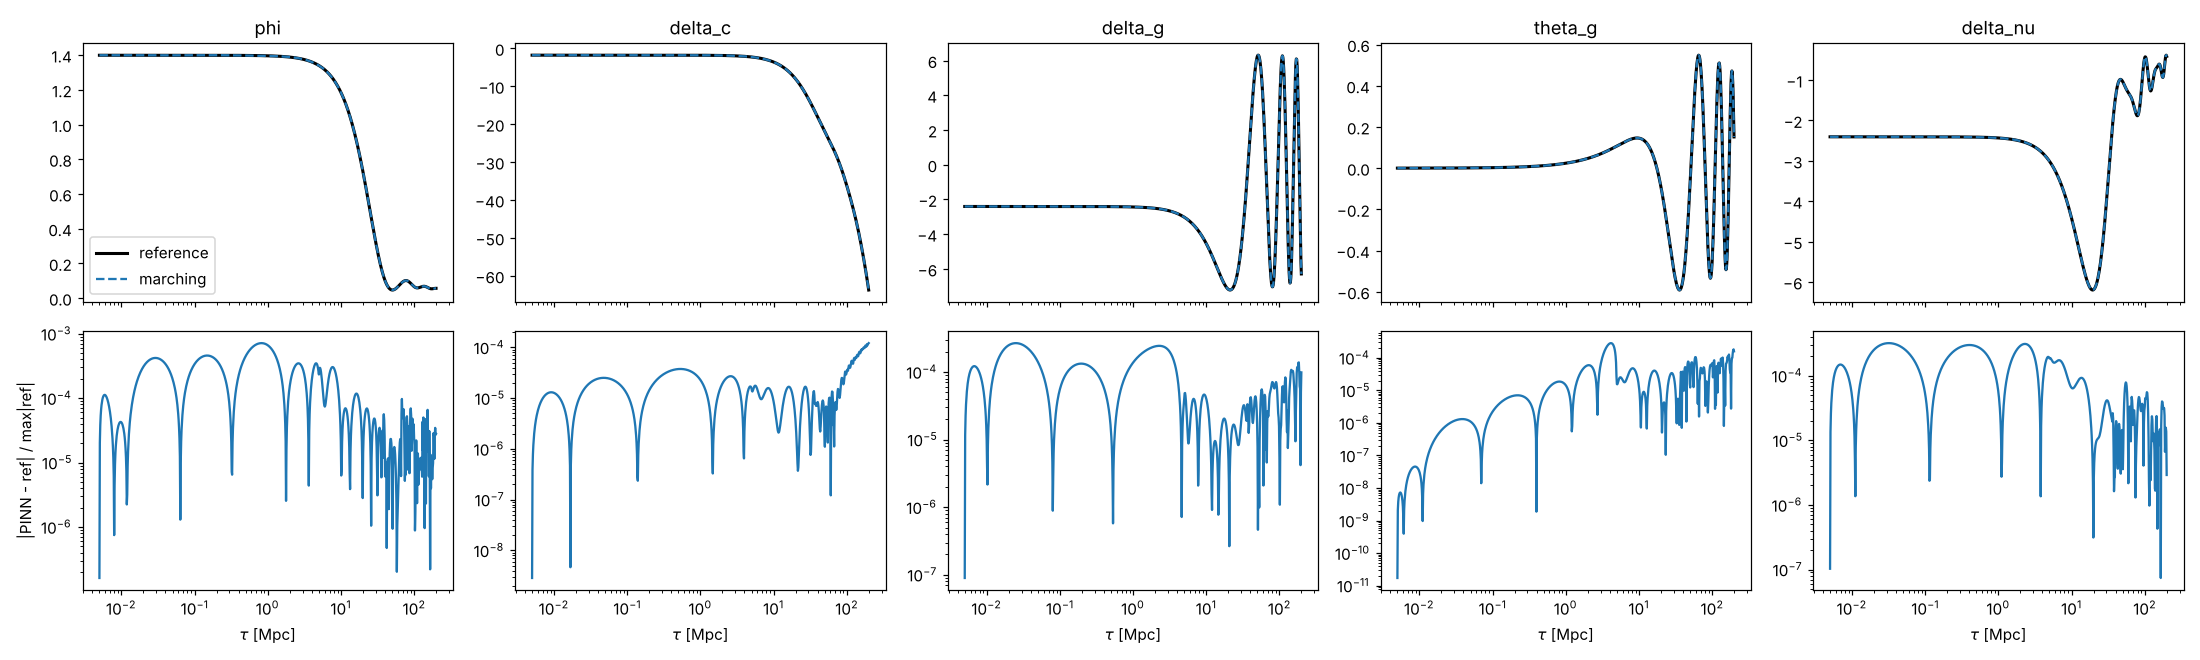
\includegraphics[width=0.49\textwidth]{figures/pilot2_marching.png}
\caption{$k=0.2$\,Mpc$^{-1}$ stress test through 3.4 acoustic oscillations. Left: a single network (with oscillation ansatz) collapses towards zero from the first time step. Right: time-marching over 8 windows; every variable is within $10^{-3}$ of the reference.}
\label{fig:pilot2}
\end{figure*}

\paragraph{The tight-coupling switch.} In a single-mode chain through recombination, the first full-hierarchy window trained to a loss of $6.7\times10^{-2}$, against $\sim5\times10^{-5}$ for every later window, when the state was handed over with zero baryon--photon slip. The full system relaxes to the quasi-static slip over $\delta\tau\sim1/\kd\approx0.01$\,Mpc, a boundary layer the network cannot represent. Handing over the first-order slip places the state on the slow manifold; the handed-over slip then matches the full system's to $10^{-4}$.

\subsection{Phase 1: wavenumber bundle in the tight-coupling era}\label{sec:phase1}

A three-window chain (edges $10^{-3}$, 1, 20, 200\,Mpc; 4$\times$64 networks with the oscillation ansatz; 20k Adam + 6k L-BFGS steps per window) was trained over $k\in[10^{-3},0.05]$\,Mpc$^{-1}$. It was evaluated on 20 held-out $k$, each up to its own TCA switch time. The RMS error over modes is $(0.9$--$2.2)\times10^{-3}$ across the variables, with maxima of $(1.7$--$5.1)\times10^{-3}$. The worst variable is the neutrino shear, and the worst mode is $k=0.033$. This misses the $10^{-3}$ target by a factor of 2--5. The error is already $\sim10^{-3}$ in the first, super-horizon window (Fig.~\ref{fig:phase1}), where the solution hardly depends on $k$. It therefore reflects accumulated residual error over a long window, not missing capacity for the $k$ dependence. Shorter windows, wider networks and second-order optimisers are the obvious remedies \pending{retrained Phase 1 chain}.

\begin{figure*}
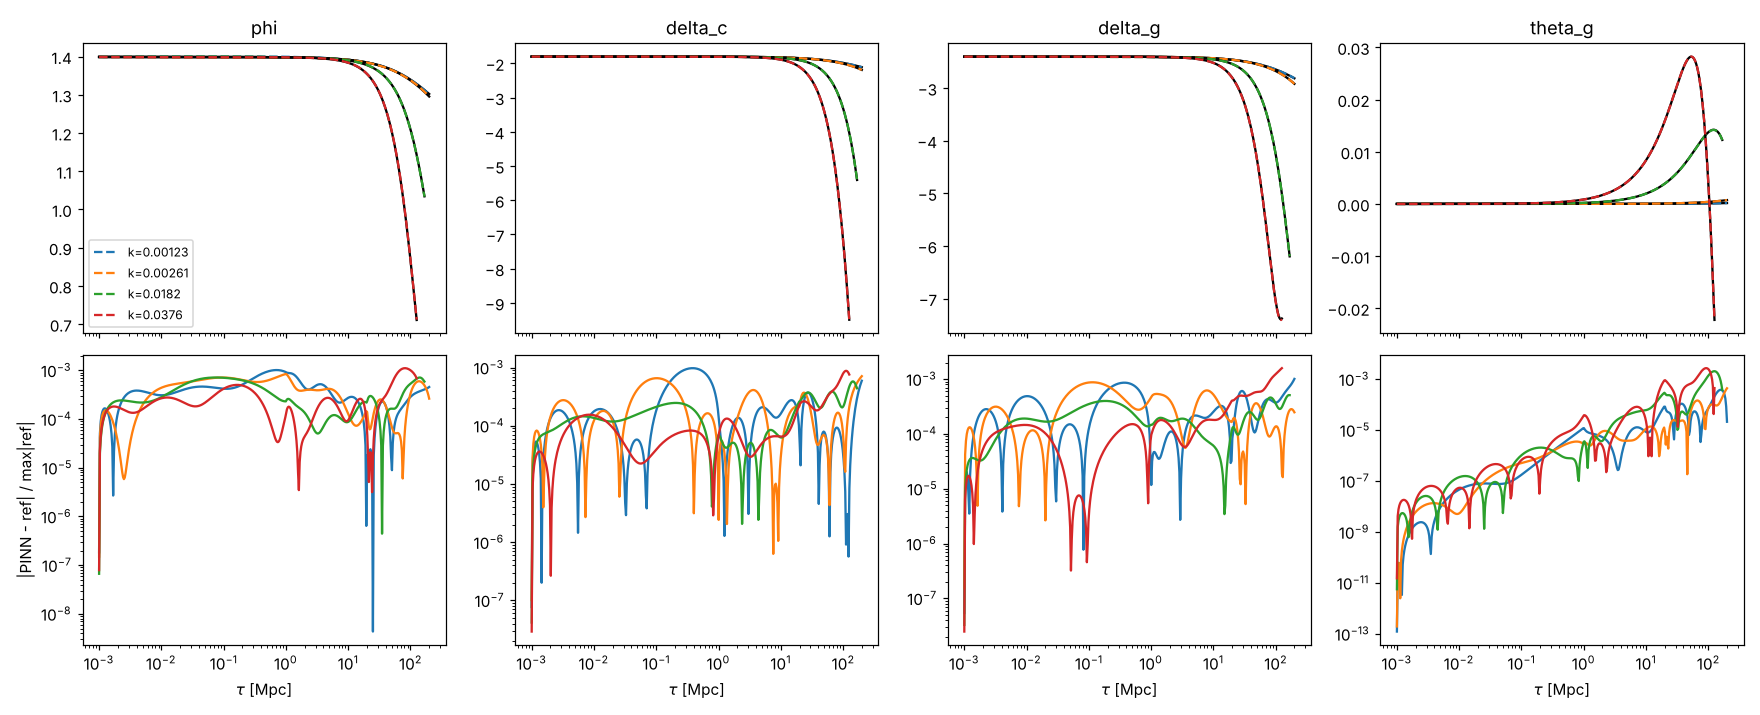
\includegraphics[width=\textwidth]{figures/phase1.png}
\caption{Phase 1 bundle over $k\in[10^{-3},0.05]$\,Mpc$^{-1}$: four of the 20 held-out modes. Bottom: error normalised by $\max|X_{\rm ref}|$.}
\label{fig:phase1}
\end{figure*}

\subsection{Phase 2: cosmological-parameter bundle}\label{sec:phase2}
\pending{bundle over $(k,\omega_b,\omega_c)\in[10^{-3},0.2]\times[0.020,0.024]\times[0.10,0.14]$ on the analytic background; held-out Latin hypercube of 30 points.}

\subsection{Phase 3: through recombination}\label{sec:phase3}
\pending{25-window chain (3 TCA, 19 full-hierarchy with $\ell_{\max}=12/10/17$, 3 per-mode RSA) over $k\in[5\times10^{-6},0.12]$\,Mpc$^{-1}$; errors against \textsc{class} up to $2\taurec$.}

\subsection{Phase 4: $C_\ell^{TT}$}\label{sec:phase4}
The approximation schedule matters before the network does. With reference-solver sources, the \textsc{class}-like schedule (TCA trigger; RSA per mode at $k\tau>45$) reproduces \textsc{class} $C_\ell^{TT}$ to $\le7.7\times10^{-3}$ for $\ell\le30$ and $\le2\times10^{-3}$ above. A $k$-independent RSA switch, which would let a bundle use fixed windows, fails at low $\ell$. Switching all modes at $\tau=850$\,Mpc gives $C_2$ wrong by a factor of 200, and at $\tau=1400$\,Mpc 13\% errors for $\ell\le5$; both are fine ($\le1\%$) above $\ell\sim30$. Low-$k$ modes never satisfy $k\tau>45$ and need the full hierarchy until today, which is why the PINN chain switches per mode. \pending{$C_\ell^{TT}$ from PINN source functions vs \textsc{class}, $\ell\le500$.}

\subsection{Phase 5: a late-time modification of gravity and an inverse problem}\label{sec:phase5}
We consider $\mu(a)=G_{\rm eff}/G=1+\mu_0\,\Omega_\Lambda(a)/\Omega_{\Lambda,0}$ multiplying $G$ in the perturbed Einstein equations, with an unchanged background. This phenomenological model is not available in standard \textsc{class}. Since $|\mu-1|<2\times10^{-5}|\mu_0|$ before $\tau=2400$\,Mpc, the Phase 3/4 chain is reused up to there, and only the later windows are retrained with $\mu_0\in[-0.5,0.5]$ as an extra input. In the reference solver, $\mu_0=0.3$ raises the comoving matter density today by $\approx1\%$ and the potential by $\approx10\%$, independently of scale. \pending{validation of the $\mu_0$ bundle; recovery of $\mu_0$ from mock $z=0$ matter and Weyl-potential spectra (1\% errors), PINN vs reference-solver likelihoods and their cost.}


%=====================================================================================
\section{Discussion}\label{sec:discussion}
%=====================================================================================

\paragraph{What generalises.} Several of the ingredients above are not specific to PINNs. The growth of the constraint-violating solution under $0i$ evolution affects any solver that evolves $\phi$ with Eq.~\eqref{eq:phidot}. It is harmless only when the initial conditions satisfy the $00$ constraint to the order of the neglected terms. For PINNs specifically, a small residual does not imply a small error in this system: the $00$ residual must be part of the loss, and it serves as a free \emph{a posteriori} diagnostic. Every failure we met (trivial solutions, the boundary layer at the TCA switch, constraint drift) is visible in the per-window losses or in $C_{00}$ without reference to the true solution.

\paragraph{Cost.} On a 4-core CPU in float64, one tight-coupling window of the $k$ bundle trains in 20--40 minutes, and the full chain to today in \pending{hours}. The reference solver integrates one mode in 5--10\,s and \textsc{class} computes $C_\ell^{TT}$ in seconds. As a forward solver for a single cosmology, the PINN is therefore not competitive with existing codes, and we do not claim otherwise. Once trained, a bundle evaluates the late-time state of a mode in milliseconds, with exact gradients with respect to $k$ and conditioning parameters. Its value lies in amortisation over many evaluations of models for which no training data exist (Sec.~\ref{sec:phase5}). We have not compared against differentiable solvers~\cite{DISCOEB,ABCMB,SymBoltz} on equal hardware \pending{benchmark}.

\paragraph{Limitations.} The present results use zeroth-order tight coupling, massless neutrinos and no reionisation, and stop at the unlensed temperature spectrum. The Phase 1 bundle misses its $10^{-3}$ target by a factor of 2--5, and the Phase 2 parameter bundle by an order of magnitude. All runs use one random seed per configuration. Residual-based error bounds~\cite{Liu2022bounds,Chantada2024bounds,GomezBachar2025} would turn the $C_{00}$ diagnostic into a certificate; extending them to this linear system is left for future work.

\paragraph{Conclusions.} \pending{to be written with the final results.}


\begin{acknowledgments}
[Acknowledgments.] This work used \textsc{class}, JAX, \texttt{optax}, \texttt{scipy} and \texttt{numpy}.
\end{acknowledgments}

\bibliography{refs}

\end{document}
